\documentclass[10pt,a4paper]{article}
\usepackage[latin1]{inputenc}
\usepackage{amsmath}
\usepackage{microtype}
\usepackage[none]{hyphenat}
\usepackage{verbatim}
\usepackage{amsfonts}
\usepackage{amssymb}
\usepackage{enumitem}
\renewcommand{\familydefault}{\sfdefault}
\usepackage{mathpazo}
\renewcommand{\rmdefault}{put}
\usepackage{enumitem}
\usepackage[dvipsnames,svgnames]{xcolor}
\usepackage{tkz-euclide}
\usetkzobj{all}
\usepackage{graphicx}
\usepackage{tikz} 	
\usepackage{adjustbox}
\usepackage{multicol}
\usepackage{lipsum}
\usepackage[left=0.7cm,right=1cm,top=1cm,bottom=1.5cm]{geometry}
\usepackage{cancel} \usepackage{xcolor}
\usepackage{tcolorbox}
\usetikzlibrary{decorations.pathmorphing,patterns}
\usetikzlibrary{decorations.pathreplacing,calc}
 \newcommand\coret[2][red]{\renewcommand\CancelColor{\color{#1}}\cancel{#2}}
\SetLabelAlign{Center}{\hfil\makebox[1.0em]{#1}\hfil}

%%_------= solusi


% Set this =0 to hide, =1 to show

% Set this =0 to hide, =1 to show
\newtcolorbox{mybox}[1][] { colframe = blue!10, colback = blue!3,boxsep=0pt,left=0.2em, coltitle = blue!20!black, title = \textbf{jawab}, #1, } 

%---------- kunci (jika 1 ) muncul
\def\tampilkunci{0}
\newcommand{\hide}[1]{\ifnum\tampilkunci=1
%
\begin{mybox}
 #1
\end{mybox}
%
\vspace{\baselineskip}\fi\ifnum\tampilkunci=0
%
\vspace{1cm}
%
\fi}



\newcommand*\cicled[1]{\tikz[baseline=(char.base)]{\node[white, shape=circle, fill=red!80,draw,inner sep=0.5pt](char){#1};}}

\newcommand*\kunci[1]{\ifnum\tampilkunci=1
%
\tikz[baseline=(char.base)]{\node[red, shape=circle,draw,inner sep=0.5pt,xshift=2pt](char){#1};}\stepcounter{enumii}
\fi\ifnum\tampilkunci=0
%
\hspace{3pt}#1\stepcounter{enumii}
%
\fi}

\newcommand*\silang[1]{\tikz[baseline=(char.base)]{
\draw[red,thick](-0.2,-0.20)--(0.2,0.2);
\draw[red,thick](-0.2,0.20)--(0.2,-0.2);
\node[black](char){#1};
}}

\newcommand*\centang[1]{\tikz[baseline=(char.base)]{
\draw[red, very thick](-0.2,0.1)--(-0.1,0)--(0.2,0.3);
\node(char){#1};
}}

\newcommand*\merah[1]{
\textcolor{red}{#1}}
\newcommand*\pilgan[1]{
\begin{enumerate}[label=\Alph*., itemsep=0pt,topsep=0pt,leftmargin=*,align=Center] #1 
\end{enumerate}}
\newcommand*\pernyataan[1]{
\begin{enumerate}[label=(\arabic*), itemsep=0pt,topsep=0pt,leftmargin=*] #1 
\end{enumerate}}

\newcommand{\pilgani}[1]{                            \vspace{-0.3cm}\begin{multicols}{2}
 \begin{enumerate}[label=\Alph*., itemsep=0pt,topsep=0pt,leftmargin=*,align=Center]#1                     \end{enumerate}
 \phantom{ini cuma sapi, wedus, dan ayam}
 \end{multicols}}
\newcommand{\spasi}{
    \vspace{-0.5cm}
\begin{tcolorbox} [boxrule=0.5pt,height=4.2cm, colback=white]

\end{tcolorbox}

}


\begin{document}


 \textbf{Pemantapan Materi UKK (Labschool)} \phantom{iang aaamengerjakan soal kuis ini }   
No callculator allowed !   $G = 6,7 \times 10^{-11}$

\begin{multicols*}{2}
\textbf{A. Usaha dan Energi}

\begin{enumerate}[noitemsep, topsep=0pt]
% no1 ---------------------
\item Benda massa 2 kg mula-mula diam. Jika benda tersebut ditarik dengan gaya 10 N dengan sudut $37^o$ terhadap arah horizontal, maka usaha setelah ditarik 10 m adalah . . .
\pilgani{
    \item 20 J
    \item 60 J
    \item [\kunci{C.}] 80 J
    \item 100 J
    \item 120 J }
\hide{ }


% no2 ---------------------
\item Benda dengan massa 2 kg mula-mula diam. Jika benda ditarik dengan gaya 10 N terhadap arah horizontal, maka usaha setelah bergerak 2 s adalah . . . .
\pilgani{
    \item [\kunci{A.}] 100 J
    \item 80 J
    \item 60 J
    \item 40 J
    \item 20 J }
\hide{ }


% no3 ------------------
\item Suatu gaya $F = (10\hat{i} + 3 \hat{j})$ digunakan untuk memindahkan barang dengan perpindahan $\vec{s} = (3\hat{i} -4\hat{j})$. Maka usaha pada keadaan tersebut adalah . . .
\pilgani{
    \item 6 J
    \item[\kunci{B.}] 18 J
    \item 24 J
    \item 30 J
    \item 42 J }
\hide{}


% no4 -------------------
\item Perhatikan gambar grafik di bawah ini, tentukan besar usaha hingga perpindahan 7 m . . . 

\begin{tikzpicture}[scale=0.7]
\draw [<->] (0,4.5) node [yshift=0.5cm,above,scale=.8]{$F$}-- (0,-2) ;
\draw [<->] (7,0) node [xshift=0.5cm,right,scale=.8]{$x$ (m)}-- (-2,0) ;
\foreach \x in {1,3,5,6}{
    \node at (\x,-0.3){\x};
}
\draw[dashed,gray] (1,0)--(1,1);
\draw[dashed,gray] (6,0)--(6,-1);
\foreach \y/\label in {-1/-2,0/0,1/2,2/4,4/8}{
    \node at (-0.2,\y){\label};
}
\draw [thick] (0,1) -- (1,1) -- (3,4) --  (5,0)--(6,-1);
\end{tikzpicture}
\pilgani{
    \item [\kunci{A.}] 19 J
    \item 20 J
    \item 18 J
    \item 17 J
    \item 16 J}
\hide{  }



% no5 ----------------------------
\item Sebuah benda bermassa 2 kg awalnya berada pada puncak dengan ketinggian $h=3R$. Jika ketinggian awal adalah 60m, kecepatan benda saat berada di puncak tertinggi loop yang memiliki jari-jari $R$ adalah

\begin{tikzpicture}[scale=0.7]
\draw [fill](0.8,6.1) circle (0.1cm);
\node at (1.2,6.1) [scale=0.7]{A};
\draw(0,0) --(0,6) -- (1,6)  sin (5,0);

\draw  plot [smooth, tension=2] coordinates { (5,0) (7,2) (5,4) };
\node at (5,4.2) [above, scale=0.7] {B};
\end{tikzpicture}
\pilgani{
    \item 10 m/s
    \item 10$\sqrt{2}$ m/s
    \item[\kunci{B.}] 20 m/s
    \item 20 $\sqrt{2}$ m/s
    \item 30 m/s
}
\hide{  }



% no6 ----------------------------
\item Benda bermassa 1 kg dilempar vertikal ke atas dengan kecepatan awal 40 m/s. Jika percepatan gravitasi bumi 10 m/s$^2$, besar kecepatan benda pada saat ketinggian 60 m adalah . . . .
\pilgani{
    \item 10 m/s
    \item [\kunci{B.}] 20 m/s
    \item 50 m/s
    \item 100 m/s
    \item 200 m/s
}
\hide{ }


% No7 -------------------------
\item Sebuah pompa air dapat menaikan 15 liter air tiap menit dari sumur yang dalamnya 6 m. Air disemburka oleh pompa ini dengan kecepatan 8 m/s. Daya pompa tersebut adalah . . . .
\pilgani{
    \item 20 W
    \item [\kunci{B.}] 15 W
    \item 25 W
    \item 27 W
    \item 30 W}
\hide{ }

% no8 ------------------------
\item Dengan menggunakan tangga, seseorang membawa beban 20 kg dari ketinggian 2 m hingga 12 m. Jika waktu yanng dilakukan adalah 25 sekon, maka daya rata-rata yang diperlukan orang itu adalah . . . 
\pilgani{
    \item 20 J
    \item 40 J
    \item [\kunci{C.}] 80 J
    \item 100 J
    \item 120 J}
\hide{  }



% no9 --------------------------------
\item Balok berada pada puncak bidang miring dengna ketinggian $h$. Perbandingan energi kinetik dan energi potensial saat meluncur hingga ketinggian $\frac{1}{6} h$ adalah . . . 
\pilgani{
    \item 1 : 6 
    \item 6 : 1
    \item 1 : 5
    \item[\kunci{D.}] 5 : 1 
    \item 1 : 1
}
\hide{ }


% no10 -------------------------------
\item Suatu pegas mempunyai konstanta pegas 800 N/m. Jika suatu anak panah dengan massa 10 gram dignakan, lalu pegas memendek sejauh 10 cm, maka kecepatan anak panah melesat adalah . . .
\pilgani{
    \item 10 m/s
    \item 20 m/s
    \item 20$\sqrt{2}$ m/s
    \item 30 m/s
    \item 40 m/s }
\hide{  }

\textbf{B. Gaya gravitasi} \\

% No 11 ----------------------------------------
\item Dua buah benda masing-masing 4 kg dan 3 kg berada pada jarak 2 m. Gaya gravitasi yang dirasakan benda tersebut adalah . . . .
	\pilgani{
	\item 6,7 $\times 10^{-11}$ N
	\item 1,34 $\times 10^{-11}$ N
	\item[\kunci{C.}] 2,01  $\times 10^{-10}$ N
	\item 3,35  $\times 10^{-10}$ N
	\item 6,7  $\times 10^{-10}$ N
	}
\hide{ \begin{align*}
	F &= G\frac{4.3}{2^2}=6,7\times 10^{-11} 3 = 2,01 \times 10^{-10}\text { N}\\
	\end{align*}}



 % no 12 --------------------------------------------------------------
 
\item Dua buah benda dengan massa tertentu pada jarak $r$ memiliki gaya gravitasi $F$. Jika kedua benda massanya dijadikan 3 kali lipat, dan jarak ke dua benda dijadikan 2 kali lipat, maka gaya yang terjadi sekarang adalah . . . .
\pilgani{
	\item $ 4 F $
	\item [\kunci{B.}]$\frac{9}{4} F$
	\item $\frac{1}{2} F$
	\item $\frac{4}{9} F $
	\item $\frac{4}{3} F$
}
\hide{
\begin{align*}
	F_1 &=G\frac{m_1.m_2}{r^2}\\
	F_2 &=G\frac{3.m_1}{m_2}{(2r)^2}=\frac{9}{4}G\frac{m_1.m_2}{r^2}=\frac{9}{4}F_1\\
	\end{align*} }


% no 13 ----------------------------------------------------
\item Dua buah benda dengan massa 2 kg dan 12,5 kg berada pada jarak 35 m. Jika ada benda ketiga diletakkan antara dua benda tersebut ($m$ = 3 kg), agar jumlah gaya adalah nol maka harus diletakkan di . . . . .
\pilgani{
	\item[\kunci{A.}] 10 m dari 12,5 kg
	\item 15 m dari 2 kg
	\item 10 m dari 2 kg
	\item 20 m dari 12,5 kg
	\item 25 m dari 2kg
	}
  \hide{
  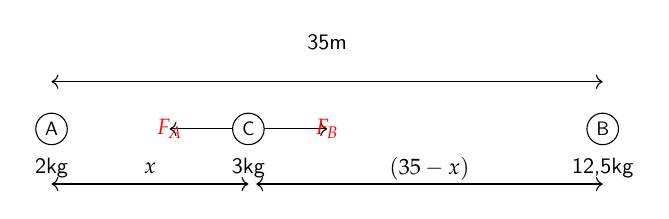
\begin{tikzpicture} 

  \foreach \x/\y/\z in {0/A/{2kg},2.5/C/{3kg},7/B/{12,5kg}} {
    \draw (\x,0) circle (0.2) node[scale=0.7] {\y};
  \node at (\x,-0.5) [scale=0.8]{\z};}
  \draw [<->] (0,0.6)--node [midway, yshift=0.5cm,scale=0.8]{35m}(7,0.6);
  \draw[<->] (0,-0.7) --node [midway, yshift=0.2cm,scale=0.8]{$x$}(2.5,-0.7);
    \draw[<->] (2.6,-0.7) --node [midway, yshift=0.2cm,scale=0.8]{$(35-x)$}(7,-0.7);
    \draw [->] (2.3,0) -- (1.5,0) node [scale=0.8, red]{$F_A$};
        \draw [->] (2.7,0) -- (3.5,0) node [scale=0.8, red]{$F_B$};
    \end{tikzpicture}
  
  Agar total gayanya nol maka besar gaya $F_A$ dan $F_B$ harus sama
  \begin{align*}
  F_A &= F_B\\
  \coret{G}\frac{m_A\coret{m_c}}{x^2} &=\coret {G}\frac{m_B.\coret{m_c}}{(35-x)^2}\\
  \frac{m_A}{m_B} &= \left (\frac{x}{35-x}\right)^2 \\
  \frac{2}{12,5}  &= \left (\frac{x}{35-x}\right)^2 \\
\frac{4}{25}   &= \left (\frac{x}{35-x}\right)^2 \\
\frac{2}{5}&=\frac{x}{35-x}\\
x&= 10 \text{ m dari A}
    \end{align*}
  }

%   ---------------------------------------------------------------------------
\item  Seorang bermassa $m$ berada di permukaan bumi dengan jari-jari bumi $R$ dan massa bumi $M$. Perbandingan gaya gravitasi yang dialami orang ketika berada di permukaan Bumi dan ketika berada pada jarak $R$ di atas permukaan Bumi adalah . . . 
\pilgani{
	\item 1 : 1 
	\item 1 : 2
	\item 2 : 1
	\item 1 : 4
	\item[\kunci{E.}] 4 : 1 }
\hide{
	$r_1$ = $R$ dan $r_2$ berada pada ketinggian $R$ dari permukaan bumi, atau $r_2=2R$ jika dihitung dari pusat (ini yang dipakai)
	\begin{align*}
	F_1 &=G\frac{Mm}{R^2}\\
	F_2 & = G\frac{Mm}{r_2^2}=G\frac{Mm}{2R^2}=\frac{1}{4} F_1\\
	F_1 : F_2 &= 1 : \frac{1}{4} =4 : 1
	\end{align*}
	}



% no B 4 ------------------------------------------------
\item Percepatan gravitasi di permukaan bumi adalah 10 N/kg. Pada titik di ketinggian tertentu percepatan gravitasi adalah 2 N/kg. Posisi tersebut dari pusat bumi adalah. . . . 
\pilgani{
	\item[\kunci{A.}]$\sqrt{5}$ R
	\item $\sqrt{2}$ R
	\item $2\sqrt{3}$ R
	\item $2\sqrt{2} $ R
	\item $\frac{1}{2} $ R
	}
\hide{
\begin{align*}
\frac{g_2}{g_1} & = \frac{M_2}{M_1}\frac{r_1^2}{r_2^2}\\
\frac{2}{10} &= \frac{\coret{M}}{\coret{M}}\frac{R^2}{r_2^2}\\
r_2^2 &= 5 R^2 \\
r_2^2 &= \sqrt{5} R\\
\end{align*}}




% No B 5  ---------------------------------------------------------------------------
\item Planet x memiliki percepatan gravitasi 7,5 kali gravitasi bumi. Jika jari-jari planet adalah 2 kali bumi, maka massa planet adalah . . . 
\pilgani{
	\item[\kunci{A.}] $30 M$ 
	\item $20 M $
	\item $10 M$
	\item $ \frac{1}{2} M$
	\item $ \frac{3}{4} M$
	}
\hide{
diketahui $g_2$ = 7,5 kali gravitasi bumi atau 7,5 $g$, dan $r_2$ = 2$r_1$. Massa planet adalah . . . 
\begin{align*}
\frac{g_2}{g_1} & = \frac{M_2}{M_1}\frac{r_1^2}{r_2^2}\\
\frac{7,5}{1} & = \frac{M_2}{M}\frac{r^2}{(2r)^2}\\
7,5 & = \frac{M_2}{4 M}\\
30 M & = M_2
\end{align*}
}


\item Suatu planet berada pada jarak 2,25 kali jarak bumi matahari. Maka waktu putaran planet tersebut mengelilingi matahari adalah . . . .
\pilgani{
    \item[\kunci{A.}] 3,375 tahun
    \item 2,25 tahun
    \item 1,5 tahun
    \item 0,5 tahun
    \item 0,25 tahun
}
\hide{
Perlu diketahui bahwa $T$ bumi adalah 1 tahun mengelilingi matahari, maka 
\begin {align*}
\left( \frac{T_2}{T_1} \right)^2 &= \left( \frac{R_2}{R_1} \right)^3 \\
\left( \frac{T_2}{1} \right)^2 &= \left( \frac{2,25}{1} \right)^3  \\
\left( \frac{T_2}{1} \right)^2 &= \left( \frac{9}{4} \right)^3  \\
\left( \frac{T_2}{1} \right) &= \left( \frac{9}{4} \right)^{\frac{3}{2}}  \\
T_2 &=\left( \frac{3}{2} \right)^{\frac{3}{\coret{2}}} \\
T_2 &= \frac{27}{8} = 3,375 \text{ tahun}
\end{align*}
}

% D. 2
\item Periode planet A dan B masing-masing 27 dan 8 tahun. Jika diketahui jarak planet B ke pusat tata surya adalah 44 juta km, maka jarak planet A ke pusat tata surya adalah . . . 
\pilgani{
    \item 23
    \item 64
    \item 81
    \item [\kunci{D.}]99
    \item 256
}
\hide{ 
\begin {align*}
\left( \frac{T_2}{T_1} \right)^2 &= \left( \frac{R_2}{R_1} \right)^3 \\
\left( \frac{27}{8} \right)^2 &= \left( \frac{R_A}{44} \right)^3 \\
\left( \frac{27}{8} \right)^{\frac{2}{3}} &= \left( \frac{R_A}{44} \right) \\
\left( \frac{3}{2} \right)^{\frac{2}{\coret{3}}} &= \left( \frac{R_A}{44} \right) \\
\frac{9}{4} &= \frac{R_A}{44}\\
99 &= R_A
\end{align*}
}
\hide{ }

\item Dua buah benda memiliki massa yang sama $m$, terpisah pada jarak $r$ sehingga menghasilkan gaya tarik menarik 10 N. Jika masing-masing benda dijadikan 2 kali massa mula-mula, dan jarak diubah menjadi 2 kalinya, maka gaya tarik menarik sekarang adalah . . .
\pilgani{
	\item 5 N
	\item 10 N
	\item 20 N
	\item 40 N
	\item 50 N}
\hide{
}

\item Berat seorang astronot adalah 800 N di bumi. Maka berat astronot tersebut di planet yang memiliki massa 3 kali bumi dan jari-jari 2 kali bumi adalah . . .
\pilgani{
	\item 100 N
	\item 400 N
	\item 600 N
	\item 900 N
	\item 1200 N }
\hide{

}
\item Planet X memiliki massa jenis 2 kali planet bumi, dan jari-jari 1,5 kali bumi. Maka besar medan gravitasi di permukaan planet X adalah . . .
\pilgani{
	\item 3 $g$
	\item 1,5 $g$
	\item 4,5 $g$
	\item 9 $g$
	\item 10,5 $g$
	}
	


\end{enumerate}


\end{multicols*}
\end{document}






